\section{Theorie}
\label{sec:Theorie}

Ziel dieses Versuches ist die Verifizierung der Fourier-Analyse und Synthese. \\

Nach dem Fourier-Theorem lassen sich zeitlich (oder räumlich) periodische Vorgänge mit der Periodendauer
$T$, für die

\begin{equation}
    f(t + T) = f(t) 
\end{equation}

gilt, durch Superposition von Sinus- und Kosinusfunktionen verschiedener Frequenzen und Amplituden genähert werden.
Dafür konvergiert die Fourierreihe

\begin{equation}
    \label{eqn:Entwicklung}
    \frac{a_0}{2} + \sum^\infty_{k = 1} \left(a_k \;  \text{cos}\left(\frac{2 \pi k t}{T} \right) + b_k \; \text{sin}
    \left(\frac{2 \pi k t}{T} \right) \right)
\end{equation}

gegen die periodische Funktion $f(t)$.   

Die sogenannten Fourierkoeffizienten $a_k$ und $b_k$ sind die Amplituden der einzelnen Sinus- und Kosinusfunktionen 
 und werden durch 

\begin{align}
    \label{eqn:Koeff}
    a_k &= \frac{2}{T} \int_0^T f(t) \; \text{cos}\left(\frac{2 \pi k t}{T} \right) \; \text{d}t \\
    b_k &= \frac{2}{T} \int_0^T f(t) \; \text{sin}\left(\frac{2 \pi k t}{T} \right) \; \text{d}t
\end{align}

mit $k \in \symbb{N}$ bestimmt. 

Diese Ermittlung der Fourierkoeffizienten $a_k$ und $b_k$ wird als Fourieranalyse bezeichnet.
Dabei verschwinden für gerade Funktionen mit $f(-t) = f(t)$ die Koeffizienten $b_k$ mit den ungeraden Sinusfunktionen und für
ungerade Funktionen mit $f(-t) = -f(t)$ die Koeffizienten $a_k$ mit geraden Kosinusfunktionen. \\

Das Frequenzspektrum der fourieranalysierten Funktion entsteht durch Auftragung der Koeffizienten als Funktionen der Frequenzen.
Da die Fourierentwicklung aus einer Summe über ganzzahlige $k$ besteht, resultiert aus ihr ein Linienspektrum, dessen
Linien gegen Null streben, da die Reihe konvergieren muss. Ein Beispiel ist in 
Abbildung \ref{fig:Beispiel} zu sehen. Man nennt ein solches Frequenzspektrum
auch einen Dirac-Kamm.

\begin{figure}
  \centering
  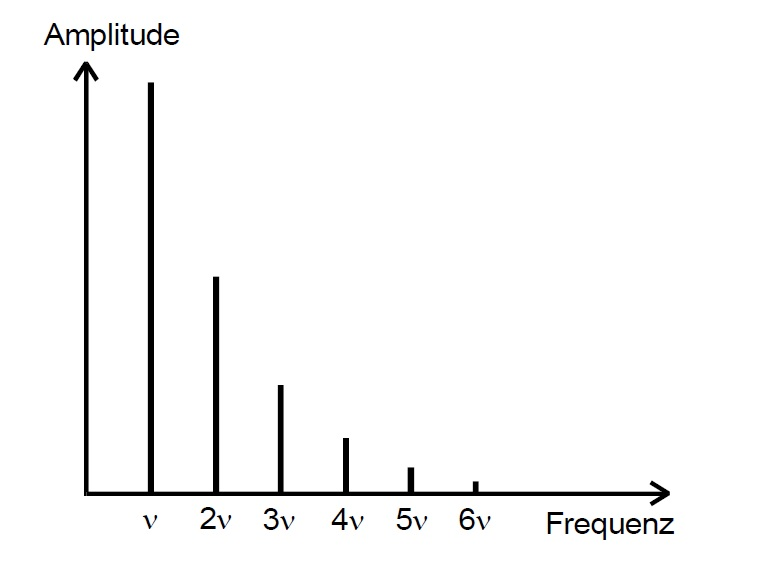
\includegraphics[scale=0.3]{content/Beispielspektrum.jpg}
  \caption{Beispiel für ein Frequenzspektrum einer periodischen Schwingung 
  mit der Grundfrequenz \mu}
  \label{fig:Beispiel}
\end{figure}

Konvergiert sie nicht, so liegt das an der Unstetigkeit der zu entwickelnden Funktion. Es tritt eine Abweichung an der Stelle
der Unstetigkeit auf, welches als Gibbsches Phänomen bezeichnet wird.

Die Fourierentwicklung \eqref{eqn:Entwicklung} enthält neben der Grundfrequenz $\nu_0 = \frac{2 \pi}{T} $ deren
ganzzahlige Vielfache - die Oberschwingungen. Außerdem können die Phasen nur $0$, $\frac{\pi}{2}$, $\pi$ oder
$\frac{3 \pi}{2}$ betragen. \\

Nichtperiodische zeitabhängige Funktionen können fouriertransformiert werden, um ihr gesamtes Frequenzspektrum bestimmen zu können.
Die Transformation

\begin{equation}
    g(\nu) = \int^\infty_{-\infty} f(t) \text{e}^{\text{i} \nu t} \; \text{d} t
\end{equation}

gibt dabei das kontinuierliche Frequenzspektrum $g(\nu)$ wieder, welches durch 

\begin{equation}
    f(t) = \frac{1}{2 \pi} \int^\infty_{-\infty} g(\nu) \text{e}^{- \text{i} \nu t} \; \text{d} \nu
\end{equation}

zurücktransformiert wird.
Im Gegensatz zur Fourierentwicklung periodischer Funktionen, resultieren hieraus in der Praxis keine perfekten
$\text{\delta}$-Funktionen, sondern Pike endlicher Breite, da die Integration über ein unendliches Intervall nicht
realisierbar ist.






